\documentclass[a4paper,11pt,oneside, titlepage]{article}
\usepackage[a4paper]{geometry} 
\geometry{a4paper,left=25mm, right=25mm, top=20mm, bottom=30mm} 
\usepackage[ngerman]{babel}
\usepackage[utf8x]{inputenc}
\usepackage[T1]{fontenc}
\usepackage{fancyhdr}
\usepackage{hyperref}
\usepackage{graphicx}
\usepackage[toc]{glossaries} 

\renewcommand{\arraystretch}{2}
\renewcommand\thesubsection{}

\pagestyle{fancy}

\lhead{\today \qquad \qquad Gruppe: na17b}
\rhead{Verantwortliche: Sieke, Gehrke, Heier, Wahsner}
\title{Testbericht\\Nachrichtenkommunikation für das THW}
\author{na17b}
\date{}

\makeglossaries
\newglossaryentry{Jest} {
  name=Jest,
  description={
    Von Facebook entwickeltes Testframework für Javascript. Zeichnet sich durch seine Einfachheit in der Benutzung aus.
  }
}
\newglossaryentry{vue-test-utils} {
  name=vue-test-utils,
  description={
    Sammlung an Funktionen um Vue-Komponenten in Unit-Tests verwenden zu können.
  }
}
\newglossaryentry{GitLab CI} {
	name=GitLab CI,
	description={
		GitLab CI ist die in GitLab eingebaute Continous Integration, die sich mit Hilfe der gitlab-ci.yml Datei konfigurieren lässt.
	}
}

\begin{document}

\maketitle

\tableofcontents

\newpage

\section{Allgemeines}
Die Tests für dieses Softwareprojekt sind eng an das Qualitätssicherungskonzept geknüpft und sollen das Funktionieren des Codes gewährleisten. Das Vorprojekt führt ausschließlich Komponententests durch, da die Kommunikation zwischen Komponenten nur indirekt über den Store erfolgt. Der Zugriff auf den Store wurde
gemocked. Als Testframework wird \gls{Jest} zusammen mit \gls{vue-test-utils} verwendet.
\section{Tests}
\subsection{Komponententests}
Komponententests befinden sich jeweils im gleichen Ordner wie die zu testende Komponente.
\subsection{GUI-Tests}
Die Testspezifikationen befinden sich vom frontend-Verzeichnis aus gesehen in \verb+test/unit/specs+.
Dort liegt für jede Komponente eine eigene Datei, welche die geforderten Eigenschaften und Funktionen
einer Komponente beschreibt. Es genügt, im Ordner frontend den Befehl \verb+npm run unit+ auszuführen; daraufhin werden alle Test-Suites automatisch abgearbeitet. Eine beispielhafte Ausgabe ist in folgender Abbildung zu sehen.
\begin{figure}[htpb]
\centering
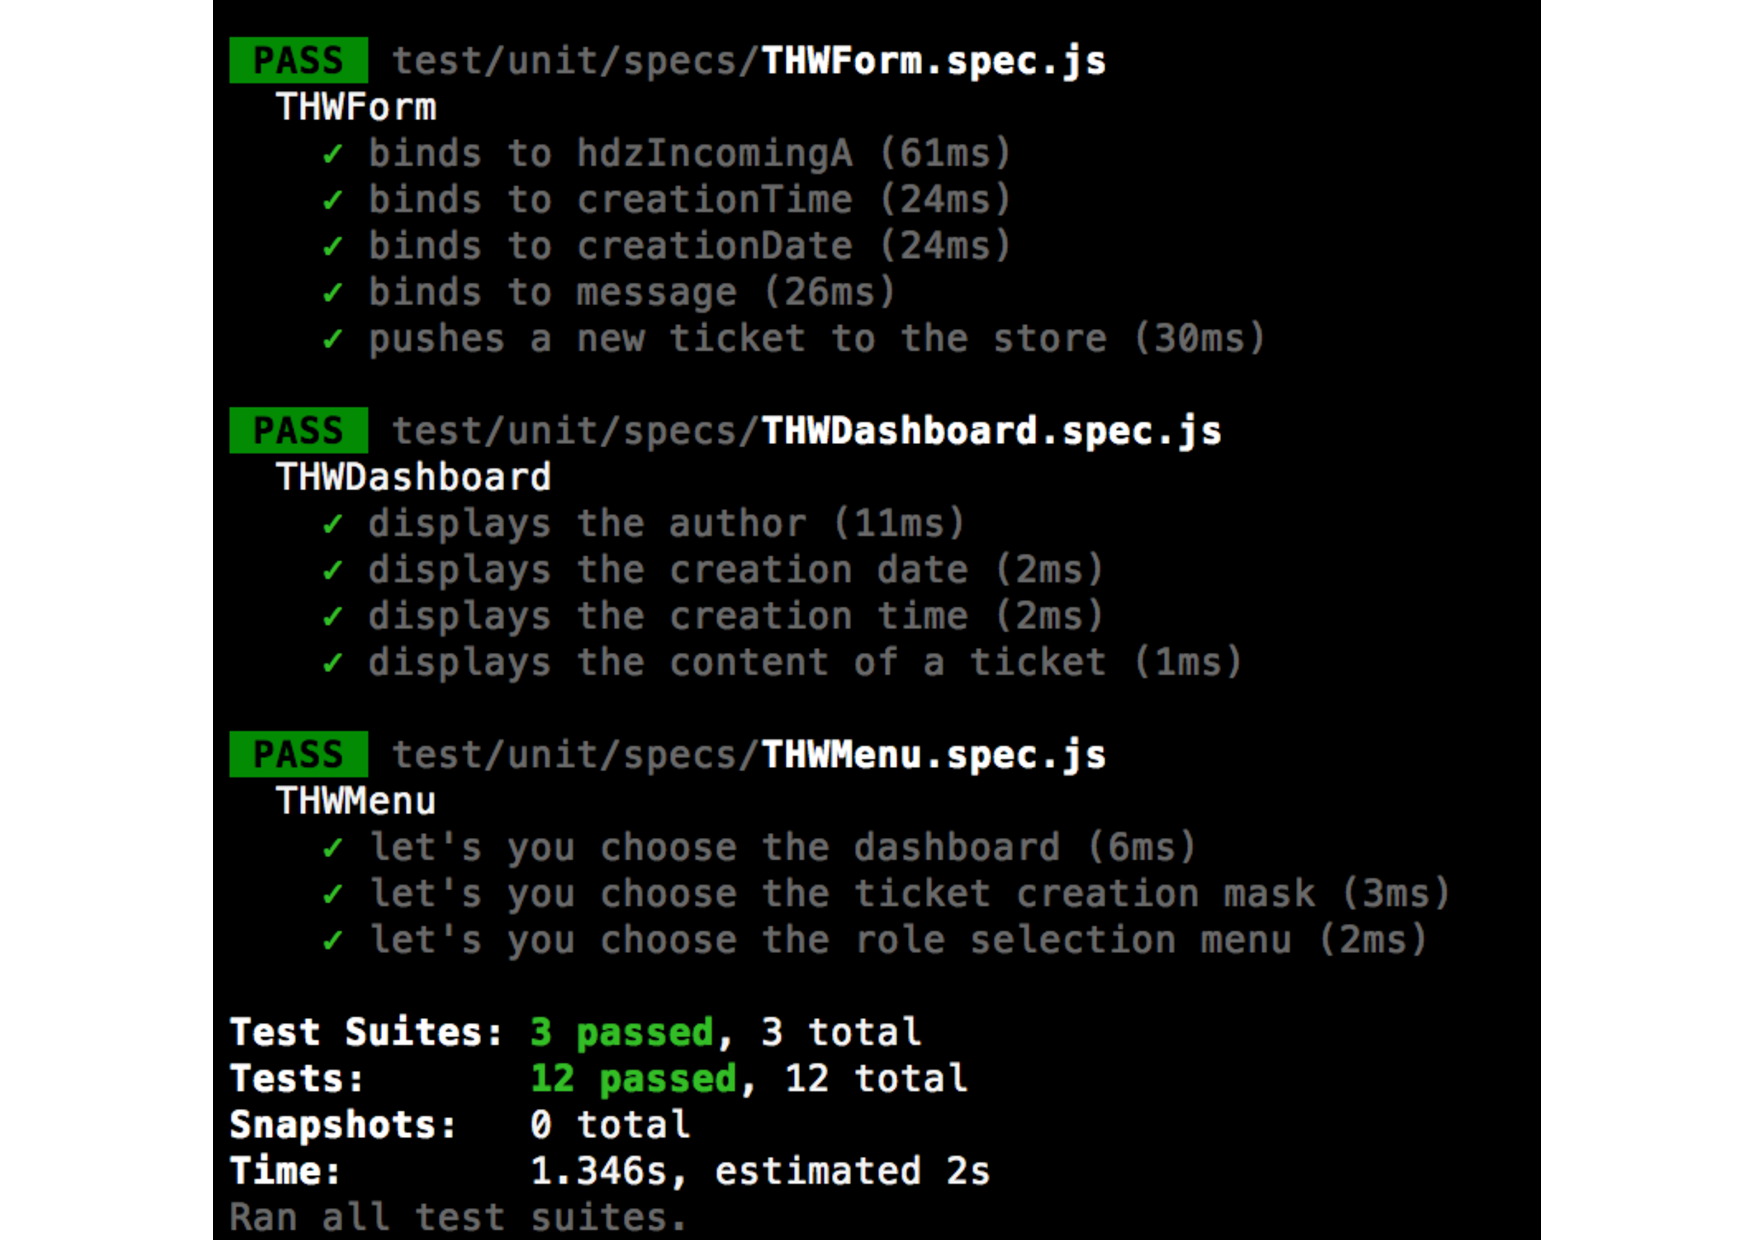
\includegraphics[width=0.8\linewidth]{testsscreenshot}
\caption{Ausgabe des Befehls npm run unit}
\label{fig:npmtest}
\end{figure}
Die Tests beschränken sich hier zunächst auf das Prüfen von Anwesenheit bestimmter Variablen und html-Elementen.
Die Ergebnisse sind in folgender Tabelle aufgelistet.
\begin{table}[htpb]
\centering
\label{tab:test}
\begin{tabular}{c | c | c}
Komponente & Anzahl Tests & Bestanden \\
\hline
THWForm & 5 & ja \\
THWDashboard & 4 & ja \\
THWMenu & 3 & ja 
\end{tabular}
\caption{Testergebnisse der momentanen Frontend-Komponenten}
\end{table}
\section{Continous Integration}
\label{sub:continous integration}
Zum zweiten Release wurde Continous Integration eingeführt, um das Einhalten der Vorgaben aus dem Dokumentationskonzept und Coding Standards automatisiert zu testen. Dazu wird GitLab CI \gls{GitLab-CI} verwendet. Die \verb+gitlab-ci.yml+ beinhaltet XML-Linting sowie JavaScript-Linting und -Testing. Um den Prozess zu beschleunigen wird auf \verb|npm install| verzichtet, stattdessen werden nur für die Tests benötigte Pakete und deren Abhängigkeiten installiert. Anschließend erfolgen linting (\verb|npm run lint|) und testing (\verb|npm run unit|).

\newpage
\printglossaries

\end{document}
